%\documentclass[11pt]{article}
\documentclass[sn-mathphys-num]{sn-jnl}

\usepackage{booktabs}

\usepackage{amssymb}
\usepackage{amsmath,amsthm}

\usepackage{hyperref}
\usepackage{xcolor}
\hypersetup{
    colorlinks,
    linkcolor={red!50!black},
    citecolor={blue!50!black},
    urlcolor={blue!80!black}
}

\usepackage{multirow}
\usepackage{pgfplots}
\usepackage{arydshln}
\usepackage{paralist}
\usepackage{booktabs}
\usepackage{pbox}

\newcounter{rqnum} %research question number
\newcommand{\rqtherqnum}{RQ`'\therqnum}
\newcommand{\rqref}[1]{RQ\ref{#1}}

\newcounter{pnum} %pain point number
\newcommand{\ppthepnum}{P`'\thepnum}
\newcommand{\ppref}[1]{P\ref{#1}}

\newcounter{qnum} %quality number
\newcommand{\qthepnum}{Q`'\theqnum}
\newcommand{\qref}[1]{Q\ref{#1}}

\newcommand{\CC}{C\nolinebreak\hspace{-.05em}\raisebox{.4ex}{\small\bf
+}\nolinebreak\hspace{-.10em}\raisebox{.4ex}{\small\bf +}}

%\pgfplotsset{compat=1.13}

% prepared for: Journal of Imaging Informatics in Medicine
% https://link.springer.com/journal/10278

\begin{document}

\title[SOP for MI Software]{State of the Practice for Medical Imaging Software
Based on Open Source Repositories}

\author*[1]{\fnm{W.\ Spencer} \sur{Smith}}\email{smiths@mcmaster.ca}

\author[1]{\fnm{Ao} \sur{Dong}}

\author[1]{\fnm{Jacques} \sur{Carette}}\email{carette@mcmaster.ca}

\author[2]{\fnm{Michael} \sur{Noseworthy}}\email{nosewor@mcmaster.ca}

\affil*[1]{\orgdiv{Computing and Software Department}, \orgname{McMaster
University}, \orgaddress{\street{1280 Main Street West}, \city{Hamilton},
\postcode{L8S 4K1}, \state{Ontario}, \country{Canada}}}

\affil[2]{\orgdiv{Electrical and Computer Engineering Department},
\orgname{McMaster University}, \orgaddress{\street{1280 Main Street West},
\city{Hamilton}, \postcode{L8S 4K1}, \state{Ontario}, \country{Canada}}}

\abstract{
We present the state of the practice for Medical Imaging (MI) software based on
data available in open source repositories. We selected 29 
projects from 48 candidates and assessed 9 software qualities (installability,
correctness/ verifiability, reliability, robustness, usability, maintainability,
reusability, understandability, and visibility/transparency) by answering 108
questions for each. Using the Analytic Hierarchy Process (AHP) on the
quantitative data, we ranked the MI software.  The top five are \textit{3D
Slicer}, \textit{ImageJ}, \textit{Fiji}, \textit{OHIF Viewer}, and
\textit{ParaView}.  This is consistent with the community's view, with four of
these also appearing in the top five using GitHub metrics (stars-per-year).  
In general, the quality and quantity of documentation present in a
project correlates quite well with its popularity.
}

\keywords{
	medical imaging, research software, software engineering, software
	quality, analytic hierarchy process}

\maketitle

\section{Introduction} \label{ch_intro}

We study the state of software development practice for Medical Imaging
(MI) software using data available in open source repositories.  MI tools use
images of the interior of the body (from sources such as Magnetic Resonance
Imaging (MRI), Computed Tomography (CT), Positron Emission Tomography (PET) and
Ultrasound) to provide critical information for diagnostic, analytic, and medical
applications. Given its importance, we want to understand the merits and
drawbacks of the current development processes, tools, and methodologies. We
use a software engineering lens to assess the quality of existing MI software.

\subsection{Research Questions} \label{sec_motivation}

As well as state of the practice (SOP) for MI software, we would like to
understand the impact of the often cited gap (chasm!) between recommended
software engineering practices and that used for most research 
software~\cite{Storer2017}. Although scientists spend
a substantial proportion of their working times on software development
\cite{Hannay2009, Prabhu2011}, few are formally trained~\cite{Hannay2009}.

Our investigation is based on the following four research questions:
\begin{enumerate}
\item[RQ\refstepcounter{rqnum}\therqnum \label{RQ_WhatProjects}:] What MI
\textbf{open source} software projects exist? (Section~\ref{ch_results})
\item [RQ\refstepcounter{rqnum}\therqnum \label{RQ_HighestQuality}:] Based on
quantitative measurements of each project's development practices, which
projects follow best practices? (Section~\ref{ch_results})
\item [RQ\refstepcounter{rqnum}\therqnum \label{RQ_CompareHQ2Popular}:] How
similar are the top projects identified in \rqref{RQ_HighestQuality}
to the most popular projects as viewed by the community?
(Section~\ref{Sec_VsCommunityRanking})
\item [RQ\refstepcounter{rqnum}\therqnum \label{RQ_CompareArtifacts}:] How
do MI projects compare to general research software with respect to the
artifacts (documents, scripts and code) present in their repositories?
(Section~\ref{Sec_CompareArtifacts})
\end{enumerate}

\subsection{Scope} \label{sec_scope}

We only cover MI visualization software.  We exclude other categories of MI
software, including Segmentation, Registration, Visualization, Enhancement,
Quantification, Simulation, plus MI archiving and telemedicine systems
(Compression, Storage, and Communication).  We also exclude Statistical Analysis
and Image-based Physiological Modelling and Feature Extraction, Classification,
and Interpretation. Software that provides MI support functions is also out of
scope; therefore, we have not assessed the toolkit libraries VTK and ITK.
Finally, Picture Archiving and Communication System (PACS), which helps users to
economically store and conveniently access images, are considered out of scope. 

\subsection{Methodology} \label{SecMethodology}

We have a standard set of questions designed to assess the qualities of any
research software project~\cite{SmithEtAl2021, SmithAndMichalski2022}.  This has
been applied to MI software and Lattice Boltzmann Solvers \cite{SmithEtAl2024}.
This builds off prior work to assess the state of the practice for such domains
as Geographic Information Systems \cite{smith2018state}, Mesh Generators
\cite{smith2016state}, Seismology software \cite{Smith2018Seismology}, and
Statistical software for psychology \cite{smith2018statistical}.  We maintain
the previous constraint that the work load for measuring a given domain should
take around one person-month's worth of effort ($20$ working days at $8$
person-hours per day).

We identify a list of potential packages (through online searches) which is then
filtered and vetted by a domain expert. We aim for roughly $30$ packages. For
each remaining package, we measure its qualities by filling in a grading
template~\cite{SmithEtAl2021}.  This data is used to rank the projects with the
Analytic Hierarchy Process (AHP).  We summarize further details on the
interaction with the domain expert, software qualities, grading the software and
AHP below and in longer form in Smith et al.\
(2024)~\cite{SmithEtAl2024_MI_SOP}.

\subsubsection{Domain Expert} \label{sec_vet_software_list}

The Domain Expert vets the proposed list because online resources can be
inaccurate.  The expert also vets the AHP ranking.  For the current assessment,
our Domain Expert is [Details of our domain expert removed for double-blind].
%%DOUBLE BLIND %our Domain Expert (and paper co-author) is Dr.\ Michael
%Noseworthy, Professor of Electrical and Computer Engineering at McMaster
%University, Co-Director of the McMaster School of Biomedical Engineering, and
%Director of Medical Imaging Physics and Engineering at St.\ Joseph's
%Healthcare, Hamilton, Ontario, Canada.  

In advance of the first meeting with the Domain Expert, they are asked to
independently create a list of top software packages in the domain.  This helps
get the expert's knowledge refreshed in advance of the meeting.

\subsubsection{Software Qualities} \label{sec_software_quality}

Quality is defined as a measure of the excellence or worth of an entity.  As is
common practice, we do not think of quality as a single measure, but rather as
a set of measures.  That is, quality is a collection of different qualities,
often called ``ilities.''  For this study we selected 9 qualities to measure:
installability, correctness/ verifiability, reliability, robustness, usability,
maintainability, reusability, understandability, and visibility/transparency.
With the exception of installability, all the qualities are defined in Ghezzi
et al. (2003) \cite{GhezziEtAl2003}. Installability is defined as the effort
required for the installation and/or uninstallation of software in a specified
environment \cite{ISO/IEC25010}.

\subsubsection{Grading} \label{sec_grading_software}

We use an existing template~\cite{SmithEtAl2021} that is designed to measure the
aforementioned qualities. To stay within our given measurement time frame, each
package gets up to five hours of time.  Project developers can be contacted for
help regarding installation, if necessary, but we impose a cap of about two
hours on the installation process.  Figure~\ref{fg_grading_template_example}
shows an excerpt of the measurement spreadsheet.  The rows are the measures and
the columns correspond to the software packages.  [The full data is available on
Mendeley; link will be provided after refereeing.] 
% \cite{Dong2021-Data}
%provides the full set of measurement data.   %%DOUBLE BLIND

\begin{figure}[!ht]
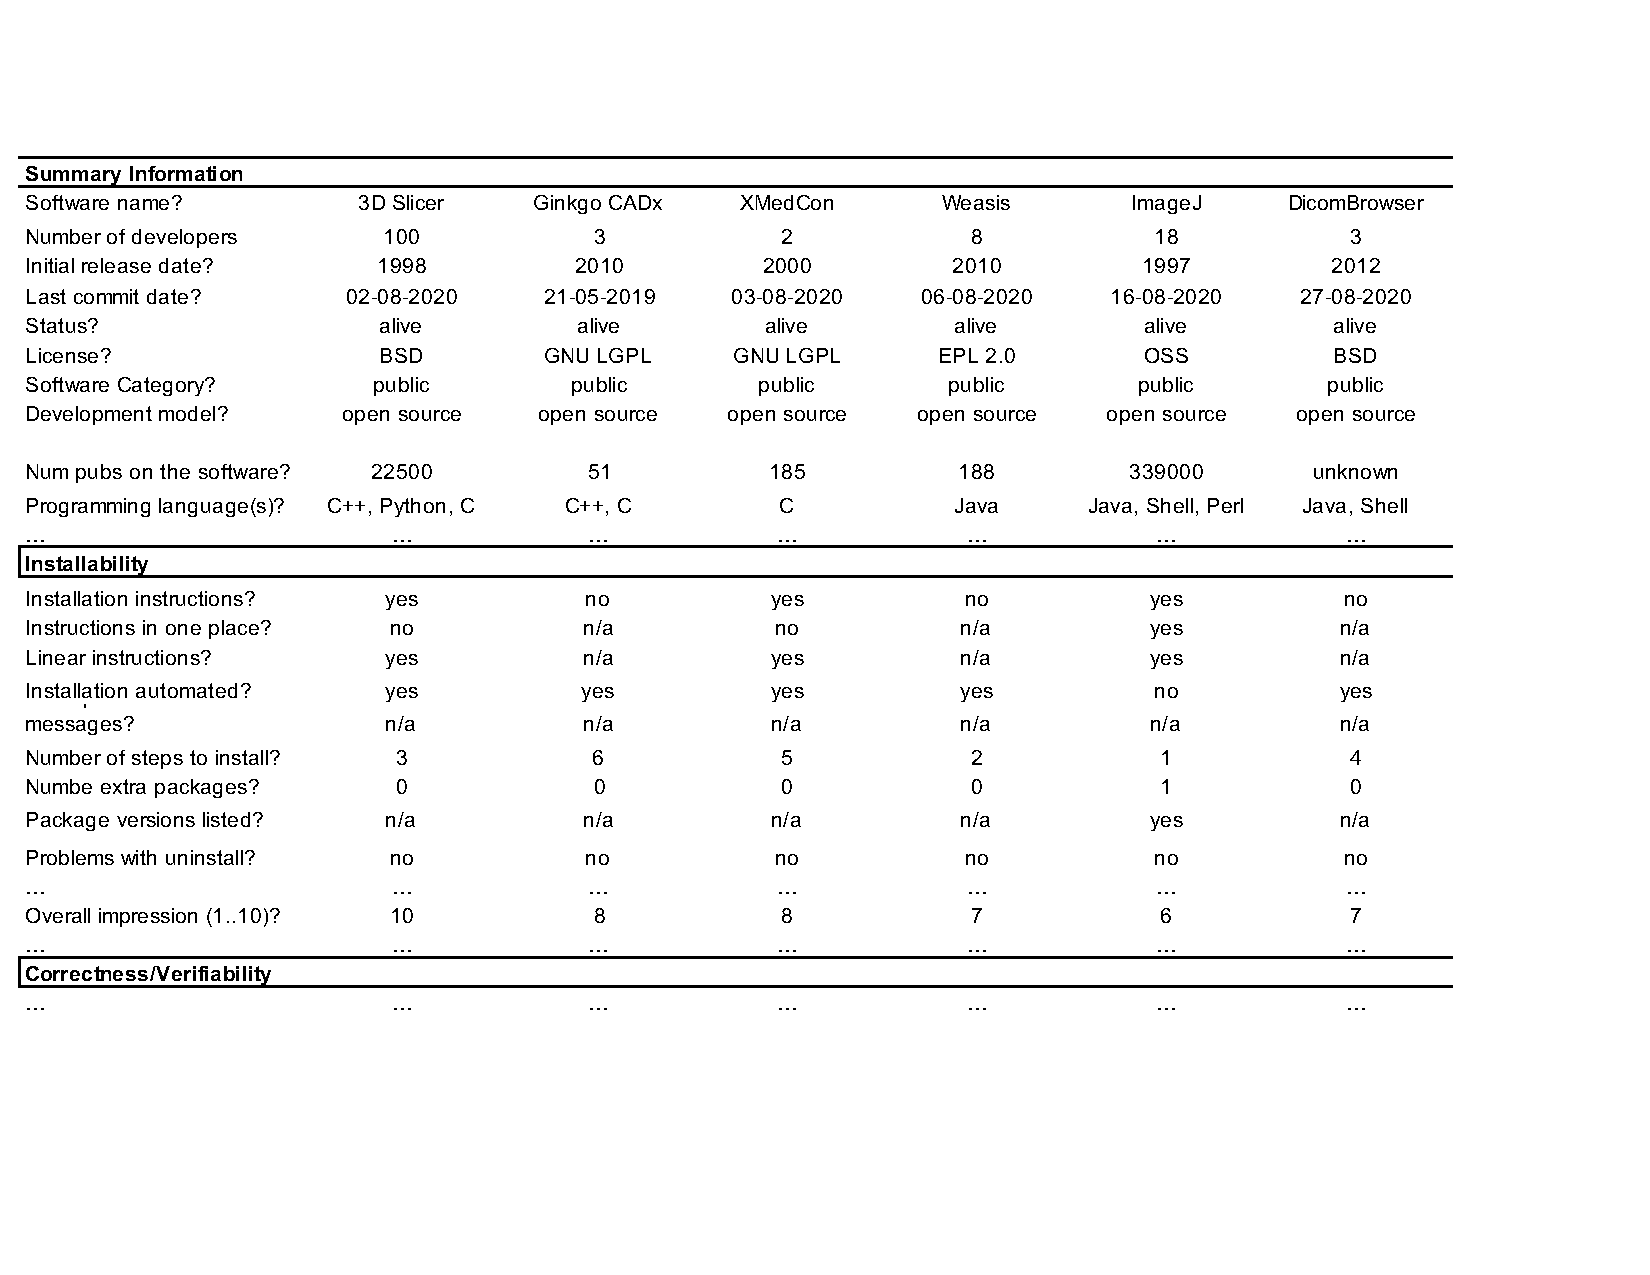
\includegraphics[scale=0.53]{template.pdf}
\caption{Grading template example}
\label{fg_grading_template_example}
\end{figure}

The full template consists of 108 questions over 9 qualities.  These
questions are designed to be unambiguous, quantifiable, and measurable
with constrained time and domain knowledge.

The grader, after answering questions for each quality assigns an overall
score (between 1 and 10) based on the answers.  Several of the qualities use
the word ``surface'' to highlight that these particular qualities are a shallow
measure.  For example, usability is not measured using user studies.
Instead, we look for signs that the developers considered usability.
We use two freeware tools to collect repository related data:
\href{https://github.com/tomgi/git_stats}{GitStats} and
\href{https://github.com/boyter/scc}{Sloc Cloc and Code (scc)}.  Further
details on quality measurement are provided in Smith et al.\ (2024)
\cite{SmithEtAl2024_MI_SOP}.

\subsubsection{Analytic Hierarchy Process (AHP)} \label{sec_AHP}

Developed by Saaty in the 1970s, AHP is widely used to analyze multiple criteria
decisions~\cite{VaidyaEtAl2006}. AHP organizes multiple criteria in a
hierarchical structure and uses pairwise comparisons between alternatives to
calculate relative ratios~\cite{Saaty1990}. AHP works with sets of $n$
\textit{options} and $m$ \textit{criteria}.  In our project $n=29$ and $m=9$
since there are 29 options (software products) and 9 criteria (qualities). With
AHP the sum of the grades (scores) for all products for a given quality will be
1.0.  We rank the software for each of the qualities, and then we combine the
quality rankings into an overall ranking based on the relative priorities
between qualities.

\section{Review} \label{ch_results}

We initially identified 48 candidate software projects from the literature
\cite{Bjorn2017, Bruhschwein2019, Haak2015}, on-line articles \cite{Emms2019,
Hasan2020, Mu2019}, and forum discussions \cite{Samala2014}.  Then we filtered
as follows:

\begin{enumerate}

\item Removed the packages with no source code available, such as
\textit{MicroDicom}, \textit{Aliza}, and \textit{jivex}.

\item Focused on MI software that provides visualization functions.  We removed
seven packages that were toolkits or libraries, such as \textit{VTK},
\textit{ITK}, and \textit{dcm4che}, and another three that were for PACS.

\item Removed \textit{Open Dicom Viewer} as it has not received any
updates since 2011.

\end{enumerate}

The Domain Expert provided a list 12 software packages.  We found 6 packages
were on both lists: \textit{3D Slicer}, \textit{Horos}, \textit{ImageJ},
\textit{Fiji}, \textit{MRIcron} (we use its descendant \textit{MRIcroGL}) and
\textit{Mango} (we use the web version \textit{Papaya}).  The remaining six
packages were on our out-of-scope list. The Domain Expert agreed with our final
choice of 29 packages -- see Table~\ref{tab_final_list}. This contains summary
data collected in the year 2020. 

The projects are sorted in descending order of lines of code.  We found the
initial release dates (Rlsd) for most projects and marked the two unknown dates
with ``?''. The date of the last update is the date of the latest update, at the
time of measurement. We found funding information (Fnd) for only eight projects.
For the Number Of Contributors (NOC) we considered anyone who made at least one
accepted commit as a contributor. The NOC is not usually the same as the number
of long-term project members, since many projects received change requests and
code from the community.  With respect to the OS, 25 packages work on all three
OSs: Windows (W), macOS (M), and Linux (L). Although the usual approach to
cross-platform compatibility was to work natively on multiple OSes, five
projects achieved platform-independence via web applications. The full
measurement data for all packages is available on [removed for blind review]
%\href{https://data.mendeley.com/datasets/k3pcdvdzj2/1} {Mendeley Data}.  
%% DOUBLE BLIND

\begin{table}[!ht]
\centering
\begin{tabular}{p{3.7cm}lllllllll}
\toprule
\multirow{2}{*}{Software} & \multirow{2}{*}{Rlsd} & \multirow{2}{*}{Updated} & \multirow{2}{*}{Fnd} & \multirow{2}{*}{NOC} & \multirow{2}{*}{LOC} & \multicolumn{3}{c}{OS} & \multirow{2}{*}{Web} \\ \cmidrule{7-9}
 &  &  &  &  &  & W & M & L &  \\ \midrule
ParaView \cite{Ahrens2005} & 2002 & 2020-10 & \checkmark & 100 & 886326 & \checkmark & \checkmark & \checkmark & \checkmark \\
Gwyddion \cite{Nevcas2012} & 2004 & 2020-11 &  & 38 & 643427 & \checkmark & \checkmark & \checkmark &  \\
Horos \cite{horosproject2020} & ? & 2020-04 &  & 21 & 561617 &  & \checkmark &  &  \\
OsiriX Lite \cite{PixmeoSARL2019} & 2004 & 2019-11 &  & 9 & 544304 &  & \checkmark &  &  \\
3D Slicer \cite{Kikinis2014} & 1998 & 2020-08 & \checkmark & 100 & 501451 & \checkmark & \checkmark & \checkmark &  \\
Drishti \cite{Limaye2012} & 2012 & 2020-08 &  & 1 & 268168 & \checkmark & \checkmark & \checkmark &  \\
Ginkgo CADx \cite{Wollny2020} & 2010 & 2019-05 &  & 3 & 257144 & \checkmark & \checkmark & \checkmark &  \\
GATE \cite{Jan2004} & 2011 & 2020-10 &  & 45 & 207122 &  & \checkmark & \checkmark &  \\
3DimViewer \cite{TESCAN2020} & ? & 2020-03 & \checkmark & 3 & 178065 & \checkmark & \checkmark &  &  \\
medInria \cite{Fillard2012} & 2009 & 2020-11 &  & 21 & 148924 & \checkmark & \checkmark & \checkmark &  \\
BioImage Suite Web \cite{Papademetris2005} & 2018 & 2020-10 & \checkmark & 13 & 139699 &
\checkmark & \checkmark & \checkmark & \checkmark \\
Weasis \cite{Roduit2021} & 2010 & 2020-08 &  & 8 & 123272 & \checkmark & \checkmark & \checkmark &  \\
AMIDE \cite{Loening2017} & 2006 & 2017-01 &  & 4 & 102827 & \checkmark & \checkmark & \checkmark &  \\
XMedCon \cite{Nolf2003} & 2000 & 2020-08 &  & 2 & 96767 & \checkmark & \checkmark & \checkmark &  \\
ITK-SNAP \cite{Yushkevich2006} & 2006 & 2020-06 & \checkmark & 13 & 88530 & \checkmark & \checkmark & \checkmark &  \\
Papaya \cite{UTHSCSA2019} & 2012 & 2019-05 &  & 9 & 71831 & \checkmark & \checkmark & \checkmark &  \\
OHIF Viewer \cite{Ziegler2020} & 2015 & 2020-10 &  & 76 & 63951 & \checkmark & \checkmark & \checkmark & \checkmark \\
SMILI \cite{Chandra2018} & 2014 & 2020-06 &  & 9 & 62626 & \checkmark & \checkmark & \checkmark &  \\
INVESALIUS 3 \cite{Amorim2015} & 2009 & 2020-09 &  & 10 & 48605 & \checkmark & \checkmark & \checkmark &  \\
dwv \cite{Martelli2021} & 2012 & 2020-09 &  & 22 & 47815 & \checkmark & \checkmark & \checkmark & \checkmark \\
DICOM Viewer \cite{Afsar2021} & 2018 & 2020-04 & \checkmark & 5 & 30761 & \checkmark & \checkmark & \checkmark &  \\
MicroView \cite{ParallaxInnovations2020} & 2015 & 2020-08 &  & 2 & 27470 & \checkmark & \checkmark & \checkmark &  \\
MatrixUser \cite{Liu2016} & 2013 & 2018-07 &  & 1 & 23121 & \checkmark & \checkmark & \checkmark &  \\
Slice:Drop \cite{Haehn2013} & 2012 & 2020-04 &  & 3 & 19020 & \checkmark & \checkmark & \checkmark & \checkmark \\
dicompyler \cite{Panchal2010} & 2009 & 2020-01 &  & 2 & 15941 & \checkmark & \checkmark &  &  \\
Fiji \cite{Schindelin2012} & 2011 & 2020-08 & \checkmark & 55 & 10833 & \checkmark & \checkmark & \checkmark &  \\
ImageJ \cite{Rueden2017} & 1997 & 2020-08 & \checkmark & 18 & 9681 & \checkmark & \checkmark & \checkmark &  \\
MRIcroGL \cite{Rorden2021} & 2015 & 2020-08 &  & 2 & 8493 & \checkmark & \checkmark & \checkmark &  \\
DicomBrowser \cite{Archie2012} & 2012 & 2020-08 &  & 3 & 5505 & \checkmark & \checkmark & \checkmark &  \\ \bottomrule
\end{tabular}
\caption{Final software list (sorted in descending order of the number of Lines
Of Code (LOC))}
\label{tab_final_list}
\end{table}

The programming languages used in order of decreasing popularity are \CC,
JavaScript, Java, C, Python, Pascal, Matlab.  The most popular language is \CC,
for 11 of 29 projects; Pascal and Matlab were each used for a single project.

\subsection{Installability} \label{sec_result_installability}

Figure \ref{fg_installability_scores} lists the installability scores.  We found
installation instructions for 16 projects, but two did not need them
(\textit{BioImage Suite Web} and \textit{Slice:Drop})
as they are web applications. 10 of the projects required extra
dependencies: Five depend on a specific browser; \textit{dwv}, \textit{OHIF
Viewer}, and \textit{GATE} needs extra libraries to build; \textit{ImageJ} and
\textit{Fiji} need an unzip tool; \textit{MatrixUser} needs Matlab;
\textit{DICOM Viewer} needs a Nextcloud platform.

\begin{figure}[!ht]
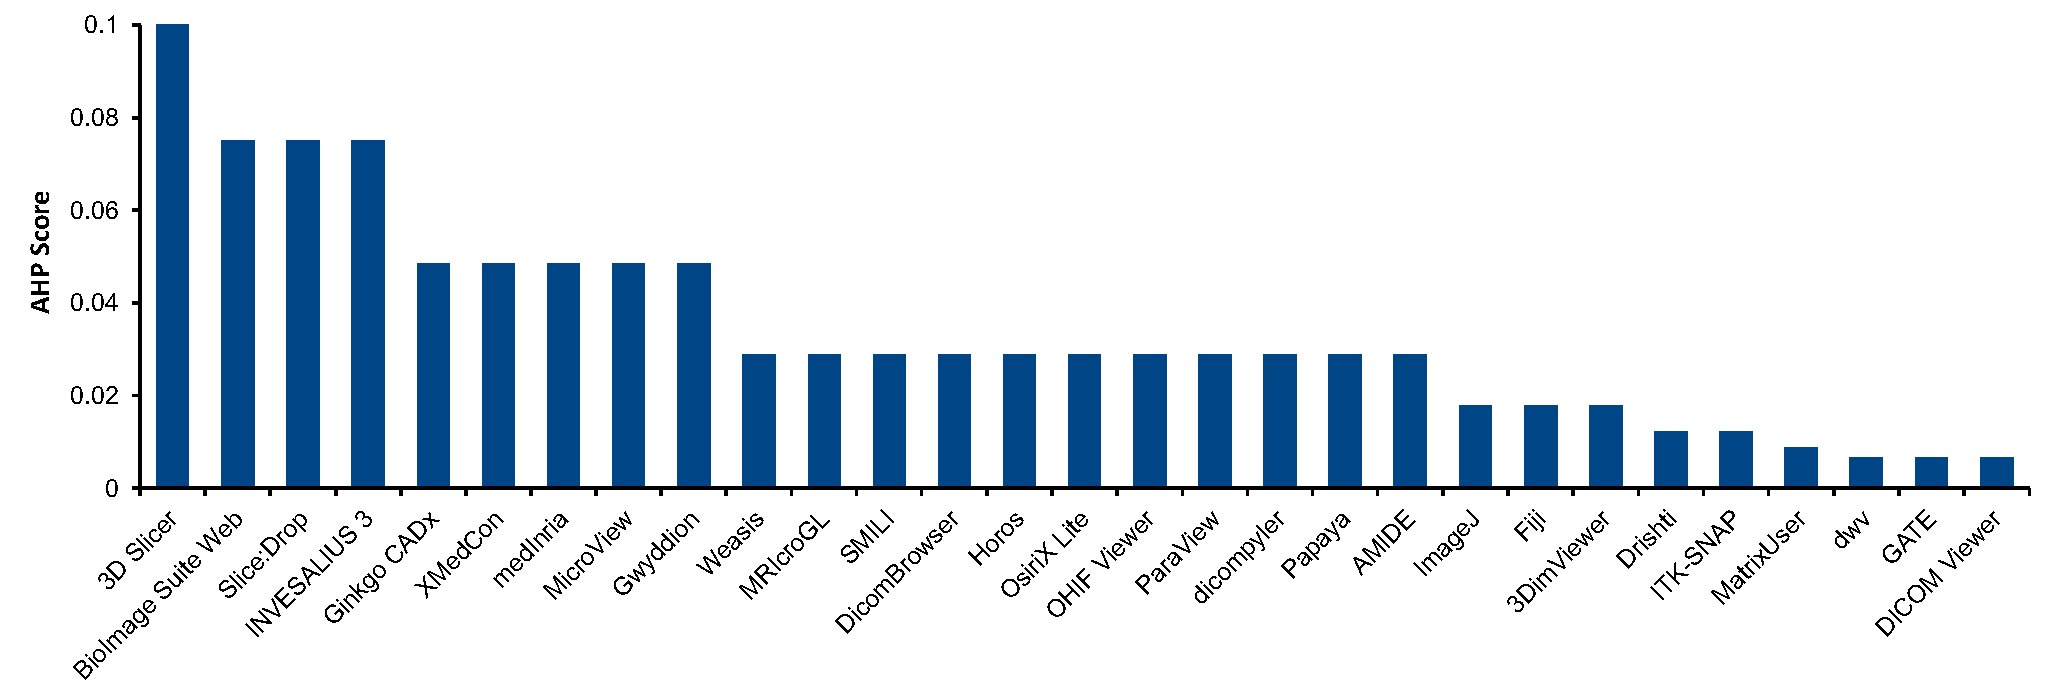
\includegraphics[scale=0.38]{installability_scores.pdf}
\caption{AHP installability scores}
\label{fg_installability_scores}
\end{figure}

The scores are based on the ease of following the installation instructions,
and automated installation and uninstallation process. There were no issues
for all but the bottom four, just various degrees of ease and automation.
\textit{GATE}, \textit{dwv}, and \textit{DICOM Viewer} showed severe
installation problems. We were not able to install them, even after a reasonable
amount of time (2 hours).  For \textit{dwv} and \textit{GATE} we failed to build
from the source code, but we were able to proceed with measuring other qualities
using a deployed on-line version for \textit{dwv}, and a virtual machine version for
\textit{GATE}. For \textit{DICOM Viewer} we could not install the NextCloud
dependency, and thus could not measure reliability nor robustness for it.

\textit{MatrixUser} depends on Matlab, whose installation is not easy.
For users who already have Matlab, this score should be higher.

\subsection{Correctness \& Verifiability} \label{sec_result_correctness_verifiability}

The packages with higher scores for correctness and verifiability (see
Figure~\ref{fg_correctness_verifiability_scores}) used a wider array of
techniques to improve correctness, and had better documentation to witness this.
For instance, we looked for evidence of unit testing, and found evidence for
only about half of the projects. We identified five projects using continuous
integration tools: \textit{3D Slicer}, \textit{ImageJ}, \textit{Fiji},
\textit{dwv}, and \textit{OHIF Viewer}. 

\begin{figure}[!ht]
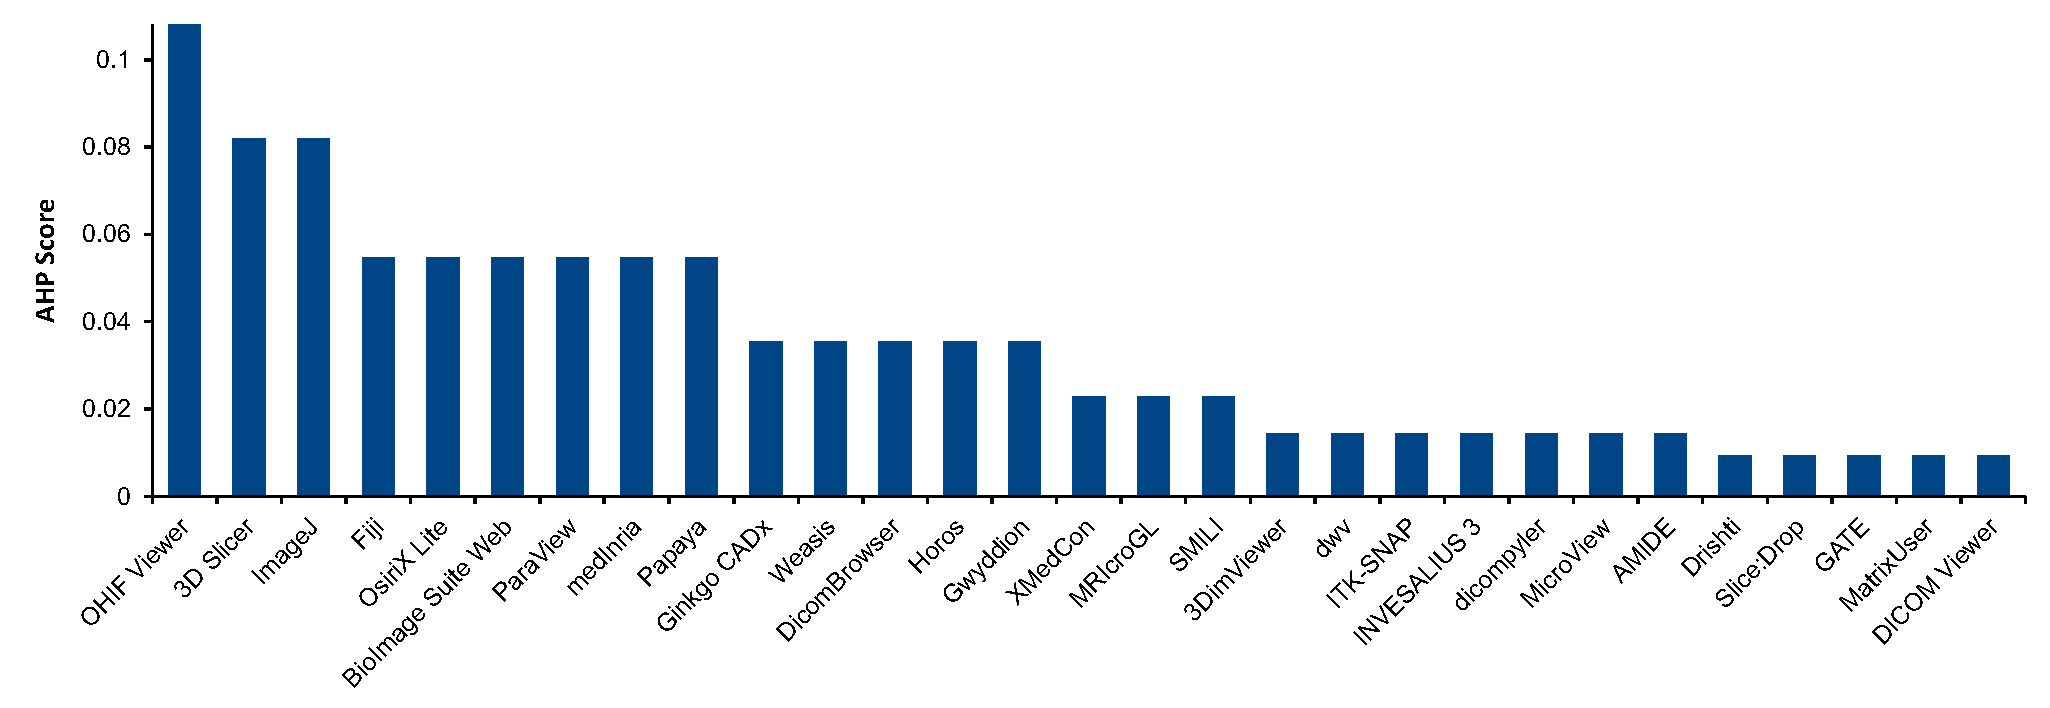
\includegraphics[scale=0.38]{correctness_verifiability_scores.pdf}
\caption{AHP correctness \& verifiability scores}
\label{fg_correctness_verifiability_scores}
\end{figure}

Even for projects with well-organized documentation, requirements
specifications and theory manuals were still missing.
The only requirements-related document we found was a road
map of \textit{3D Slicer}, which contained design requirements for upcoming
changes.

\subsection{Surface Reliability} \label{sec_result_reliability}

Figure~\ref{fg_reliability_scores} shows our results.  We were able to follow
the steps in the tutorials that existed (seven packages had them.) However,
\textit{GATE} could not open macro files and became unresponsive several times,
without any descriptive error message. We found that \textit{Drishti} crashed
when loading damaged image files, without showing any descriptive error message.

\begin{figure}[!ht]
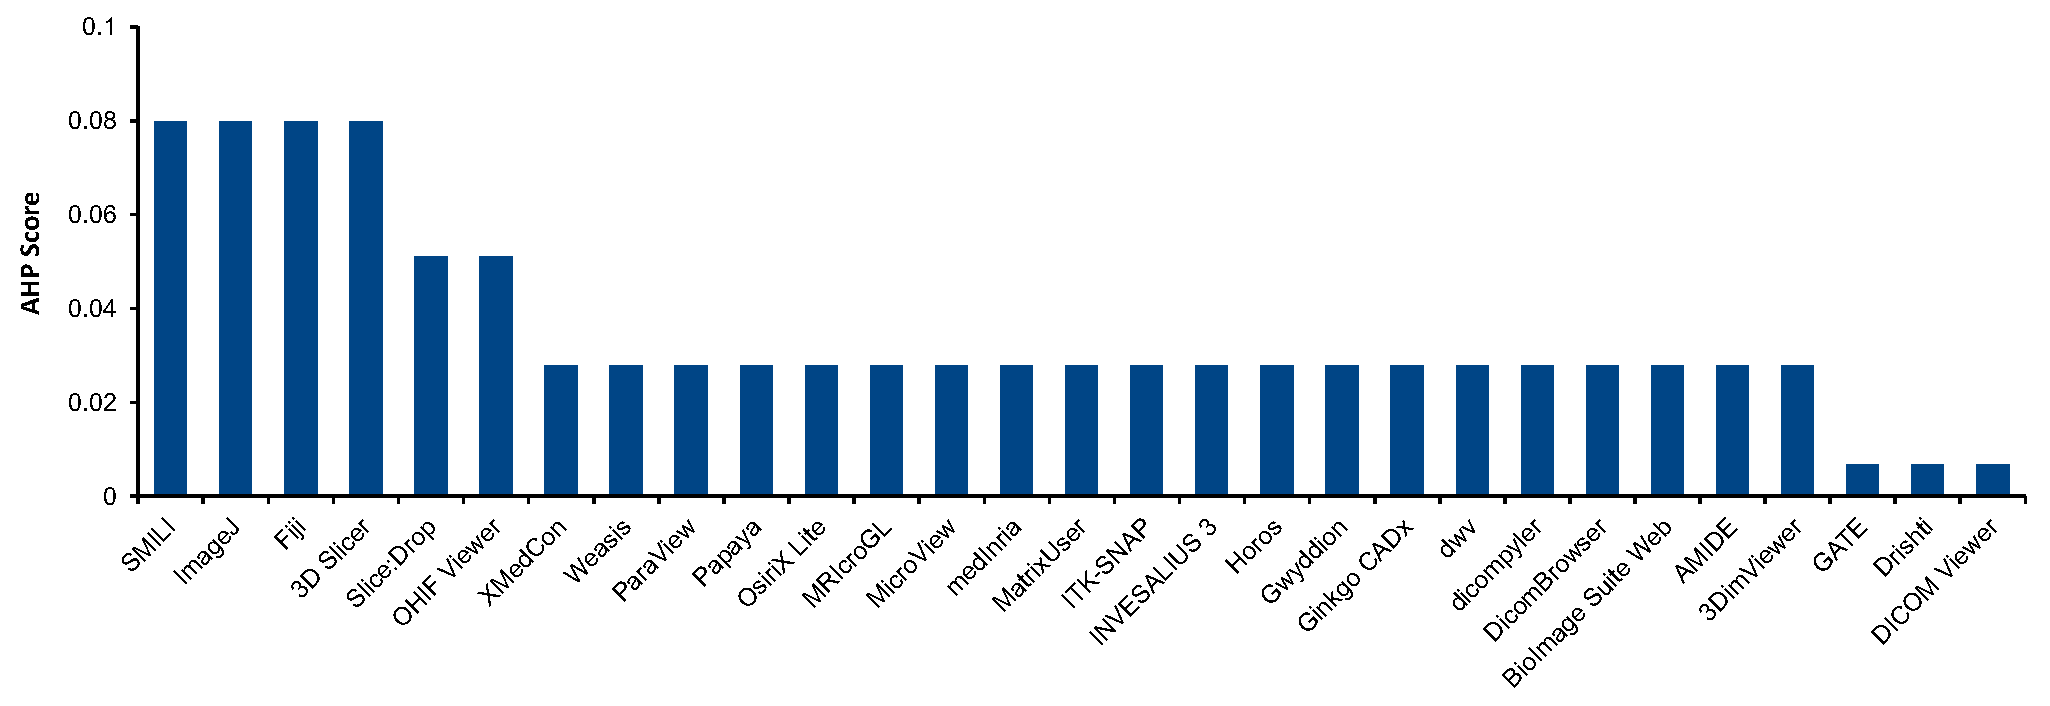
\includegraphics[scale=0.38]{reliability_scores.pdf}
\caption{AHP surface reliability scores}
\label{fg_reliability_scores}
\end{figure}

\subsection{Surface Robustness} \label{sec_result_robustness}

Figure \ref{fg_robustness_scores} presents the scores for surface robustness.
The packages with higher scores gracefully handled unexpected or unanticipated
inputs, typically showing a clear error message. We may have underscored
\textit{OHIF Viewer}, since we needed further customization to load
data.

\begin{figure}[!ht]
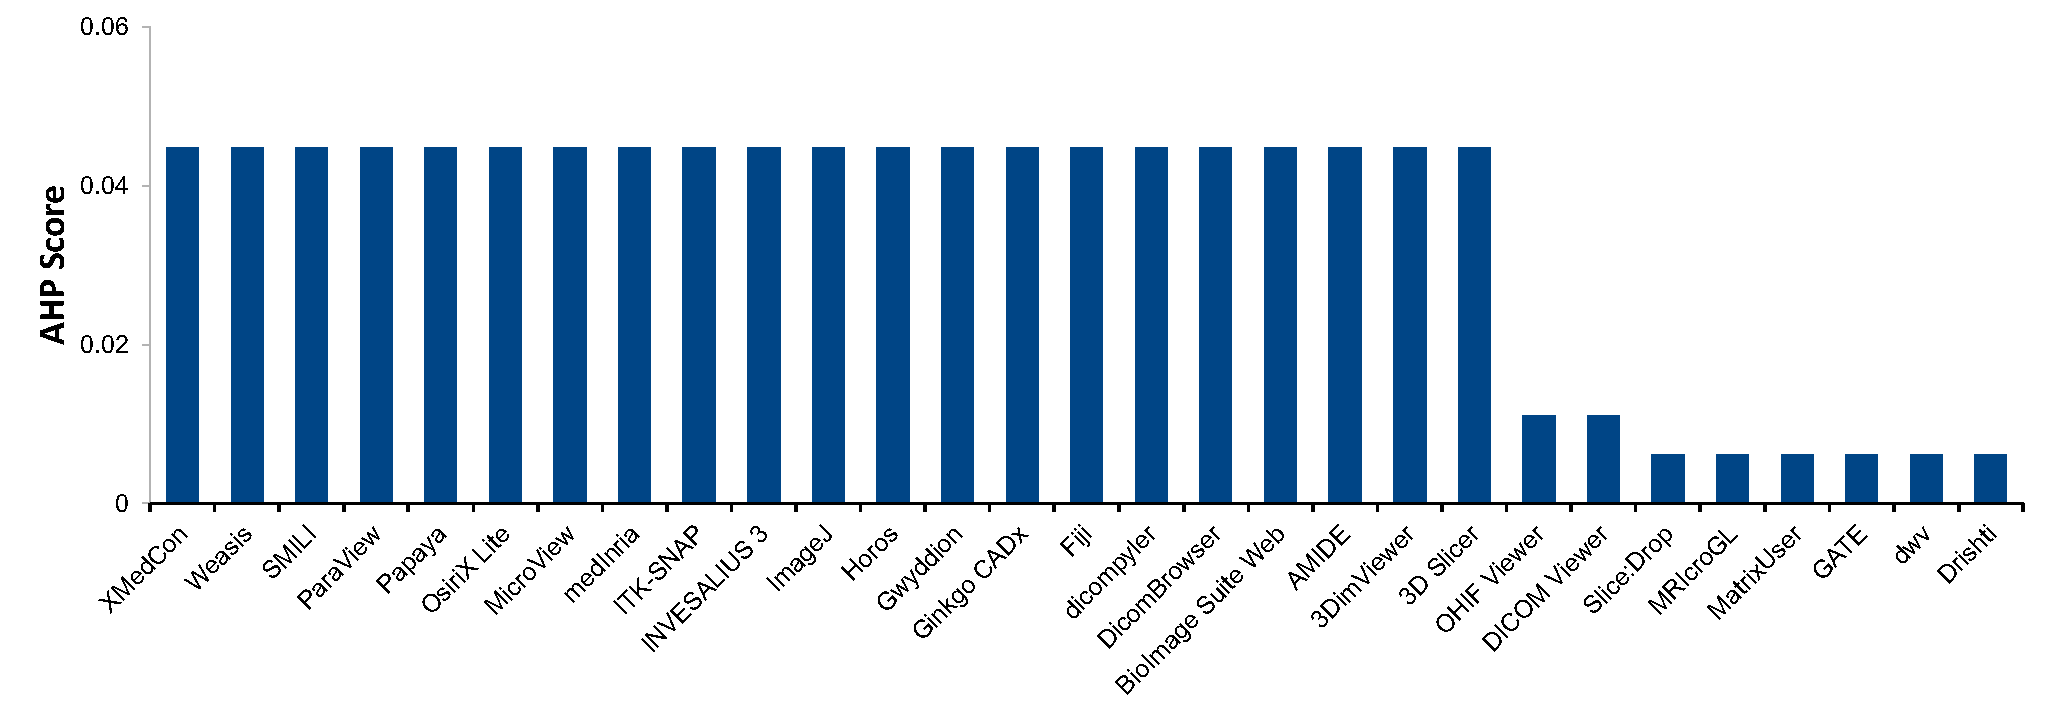
\includegraphics[scale=0.38]{robustness_scores.pdf}
\caption{AHP surface robustness scores}
\label{fg_robustness_scores}
\end{figure}

According to their documentation, all 29 software packages should support the
DICOM standard. To test robustness, we prepared two types of image files:
correct and incorrect formats (with the incorrect format created by relabelling a
text file to have the ``.dcm'' extension).  All software packages loaded the
correct format image, except for \textit{GATE}, which failed for unknown
reasons.  For the broken format, \textit{MatrixUser}, \textit{dwv}, and
\textit{Slice:Drop} ignored the incorrect format,
did not show any error message and displayed a blank image.
\textit{MRIcroGL} behaved similarly except that it showed a meaningless image.
\textit{Drishti} successfully detected the broken format of the file, but the
software crashed as a result.

\subsection{Surface Usability} \label{sec_result_usability}

Figure~\ref{fg_usability_scores} shows the AHP scores for surface usability. The
software with higher scores usually provided both comprehensive documented
guidance and a good user experience. \textit{INVESALIUS 3} provided an excellent
example of a detailed and precise user manual. \textit{GATE} also provided
numerous documents, but unfortunately we had difficulty understanding and using
them. We found getting started tutorials for only 11 projects, but a user manual
for 22 projects. \textit{MRIcroGL} was the only project that explicitly
documented expected user characteristics.

\begin{figure}[ht]
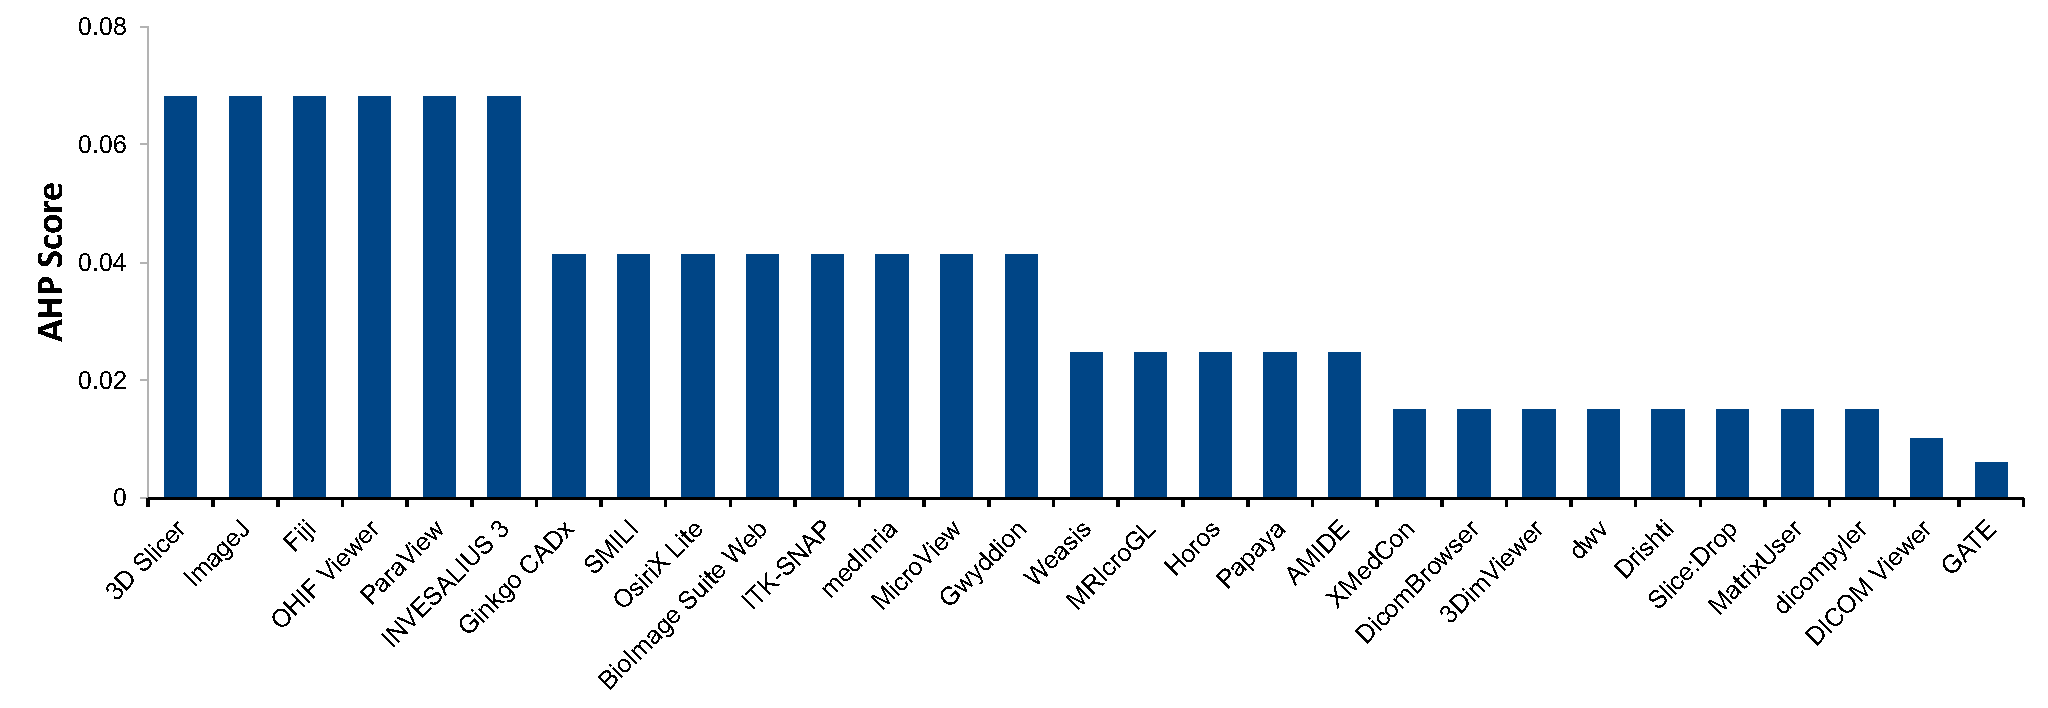
\includegraphics[scale=0.38]{usability_scores.pdf}
\caption{AHP surface usability scores}
\label{fg_usability_scores}
\end{figure}
 
\subsection{Maintainability} \label{sec_score_maintainability}

Figure~\ref{fg_maintainability_scores} shows the ranking results for
maintainability. We gave \textit{3D Slicer} the highest score because we found
it had the most comprehensive artifacts. Only a few of the 29 projects had a
product, developer's manual, or API (Application Programming Interface)
documentation, and only \textit{3D Slicer}, \textit{ImageJ}, \textit{Fiji}
included all three documents (see Table~\ref{tab_maintainability_docs} for the
full data).  Moreover, \textit{3D Slicer} has a much higher percentage of closed
issues (92\%) compared to \textit{ImageJ} (52\%) and \textit{Fiji} (64\%).

\begin{figure}[ht]
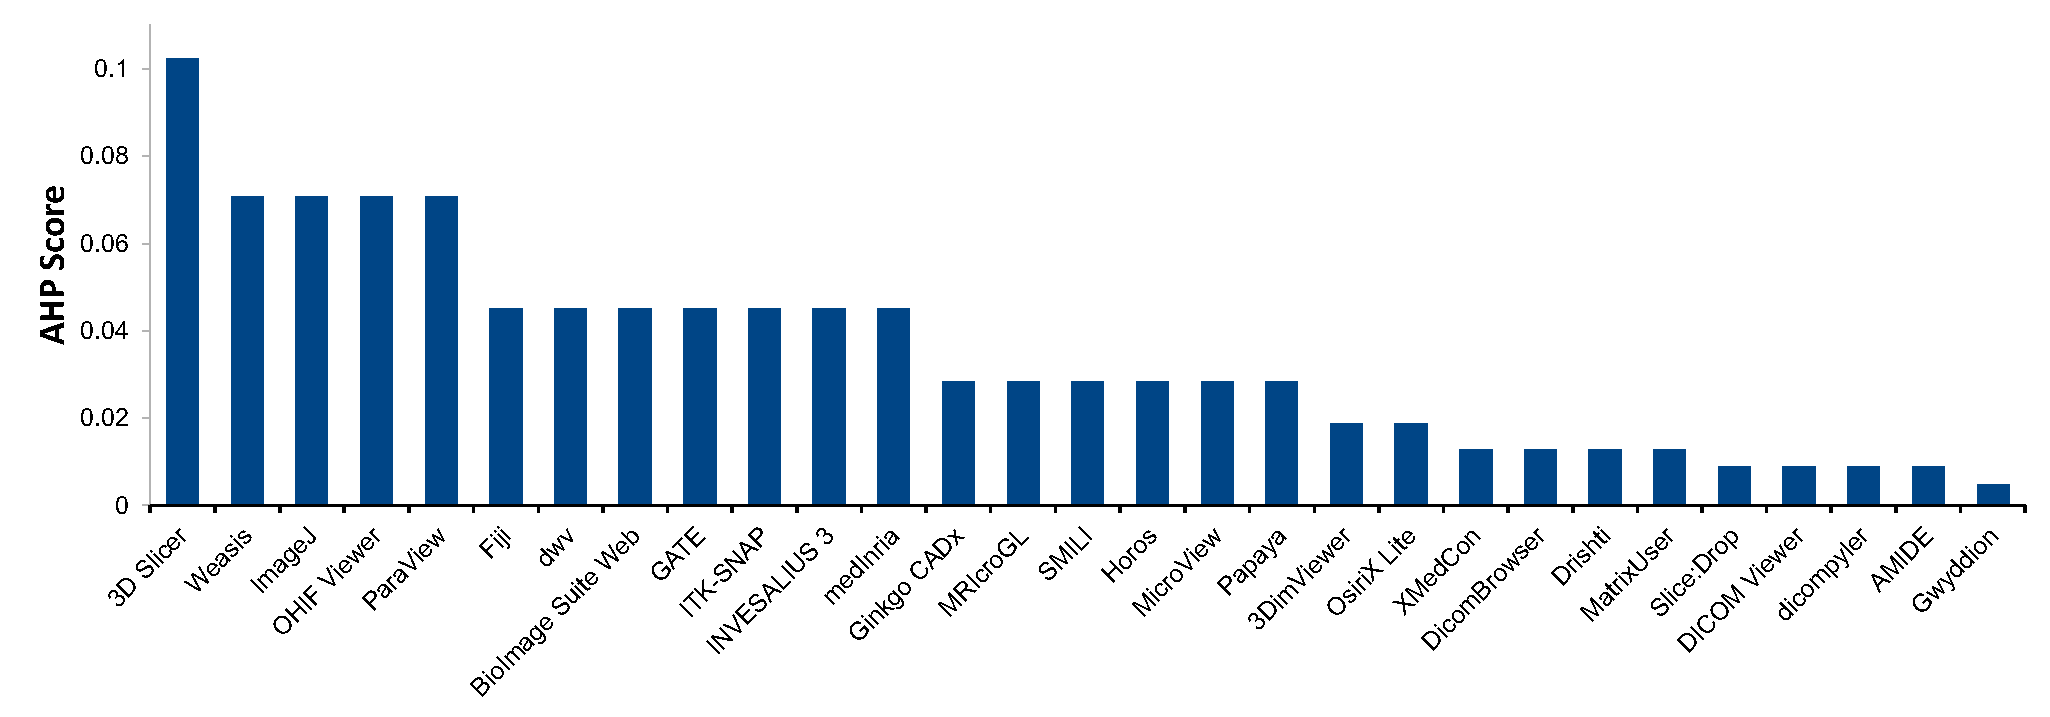
\includegraphics[scale=0.38]{maintainability_scores.pdf}
\caption{AHP maintainability scores}
\label{fg_maintainability_scores}
\end{figure}

\begin{table}[ht]
\centering
\begin{tabular}{lccc}
\toprule
\multicolumn{1}{c}{Software} & Prod.\ Roadmap & Dev.\ Manual & API Doc. \\ 
\midrule
3D Slicer & \checkmark & \checkmark & \checkmark \\
ImageJ & \checkmark & \checkmark & \checkmark \\
Weasis &  & \checkmark &  \\
OHIF Viewer &  & \checkmark & \checkmark \\
Fiji & \checkmark & \checkmark & \checkmark \\
ParaView & \checkmark &  &  \\
SMILI &  &  & \checkmark \\
medInria &  & \checkmark &  \\
INVESALIUS 3 & \checkmark &  &  \\
dwv &  &  & \checkmark \\
BioImage Suite Web &  & \checkmark &  \\
Gwyddion &  & \checkmark & \checkmark \\ 
\bottomrule
\end{tabular}
\caption{Software with the maintainability documents (listed in descending order of 
maintainability score)}
\label{tab_maintainability_docs}
\end{table}

Twenty-seven of the 29 projects used git for version control, with 24 of
these using GitHub. \textit{AMIDE} used Mercurial and \textit{Gwyddion} used
Subversion. \textit{XMedCon}, \textit{AMIDE}, and \textit{Gwyddion} used
SourceForge. \textit{DicomBrowser} and \textit{3DimViewer} used BitBucket. 

\subsection{Reusability} \label{sec_result_reusability}

API documents (see Table~\ref{tab_maintainability_docs}) also help
maintainability, which explains some of the scores shown in
Figure~\ref{fg_reusability_scores}. We have assumed that smaller code files are
likely more reusable -- see Table \ref{tab_loc_per_file} for the details.

\begin{figure}[ht]
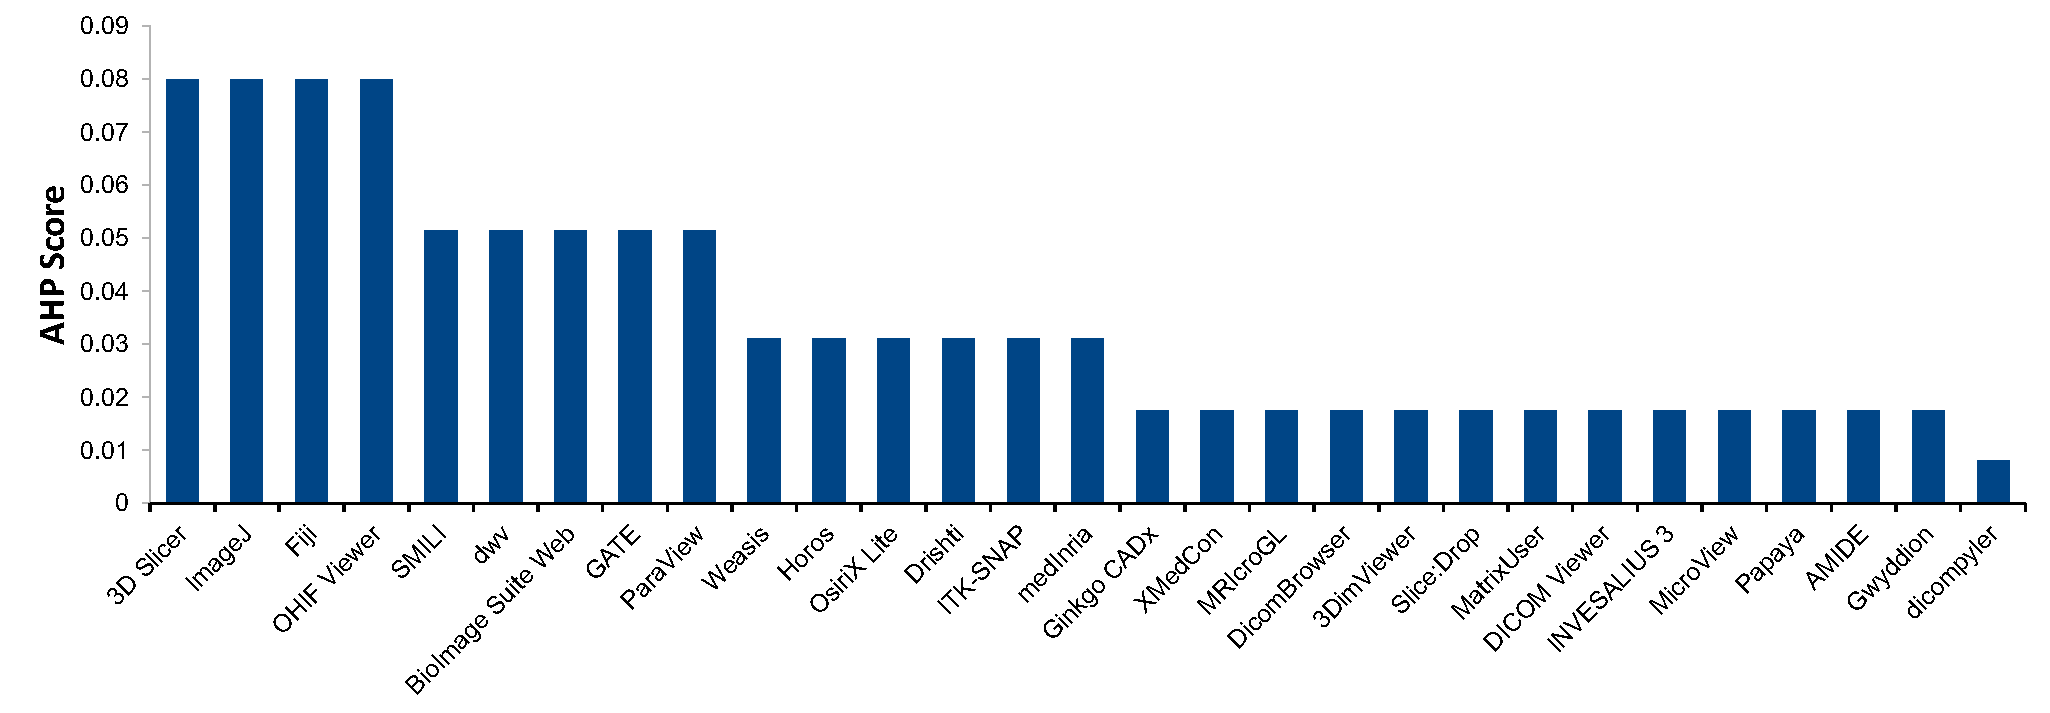
\includegraphics[scale=0.38]{reusability_scores.pdf}
\caption{AHP reusability scores}
\label{fg_reusability_scores}
\end{figure}

\begin{table}[ht]
\centering
\begin{tabular}{lllll}
\toprule
\multirow{2}{*}{Software} & \multirow{2}{*}{Text Files} & \multirow{2}{*}{Total Lines} & \multirow{2}{*}{LOC} & \multirow{2}{*}{LOC/file} \\
 &  &  &  &  \\ 
\midrule
OHIF Viewer & 1162 & 86306 & 63951 & 55 \\
3D Slicer & 3386 & 709143 & 501451 & 148 \\
Gwyddion & 2060 & 787966 & 643427 & 312 \\
ParaView & 5556 & 1276863 & 886326 & 160 \\
OsiriX Lite & 2270 & 873025 & 544304 & 240 \\
Horos & 2346 & 912496 & 561617 & 239 \\
medInria & 1678 & 214607 & 148924 & 89 \\
Weasis & 1027 & 156551 & 123272 & 120 \\
BioImage Suite Web & 931 & 203810 & 139699 & 150 \\
GATE & 1720 & 311703 & 207122 & 120 \\
Ginkgo CADx & 974 & 361207 & 257144 & 264 \\
SMILI & 275 & 90146 & 62626 & 228 \\
Fiji & 136 & 13764 & 10833 & 80 \\
Drishti & 757 & 345225 & 268168 & 354 \\
ITK-SNAP & 677 & 139880 & 88530 & 131 \\
3DimViewer & 730 & 240627 & 178065 & 244 \\
DICOM Viewer & 302 & 34701 & 30761 & 102 \\
ImageJ & 40 & 10740 & 9681 & 242 \\
dwv & 188 & 71099 & 47815 & 254 \\
MatrixUser & 216 & 31336 & 23121 & 107 \\
INVESALIUS 3 & 156 & 59328 & 48605 & 312 \\
AMIDE & 183 & 139658 & 102827 & 562 \\
Papaya & 110 & 95594 & 71831 & 653 \\
MicroView & 137 & 36173 & 27470 & 201 \\
XMedCon & 202 & 129991 & 96767 & 479 \\
MRIcroGL & 97 & 50445 & 8493 & 88 \\
Slice:Drop & 77 & 25720 & 19020 & 247 \\
DicomBrowser & 54 & 7375 & 5505 & 102 \\
dicompyler & 48 & 19201 & 15941 & 332 \\ 
\bottomrule
\end{tabular}
\caption{Number of files and lines (by reusability scores)}
\label{tab_loc_per_file}
\end{table}

\subsection{Surface Understandability} \label{sec_result_understandability}

Figure~\ref{fg_surface_understandability_scores} shows the scores for surface
understandability. 
All projects had a consistent coding style with parameters in
the same order for all functions, modularized code, and, clear comments that
indicate what is done, not how. However, we only found explicit identification
of a coding standard for 3 out of the 29: \textit{3D Slicer}, \textit{Weasis},
and \textit{ImageJ}. We also found hard-coded constants (rather than symbolic
constants) in \textit{medInria}, \textit{dicompyler}, \textit{MicroView}, and
\textit{Papaya}. We did not find any reference to the algorithms used in
projects \textit{XMedCon}, \textit{DicomBrowser}, \textit{3DimViewer},
\textit{BioImage Suite Web}, \textit{Slice:Drop}, \textit{MatrixUser},
\textit{DICOM Viewer}, \textit{dicompyler}, and \textit{Papaya}. 

\begin{figure}[ht]
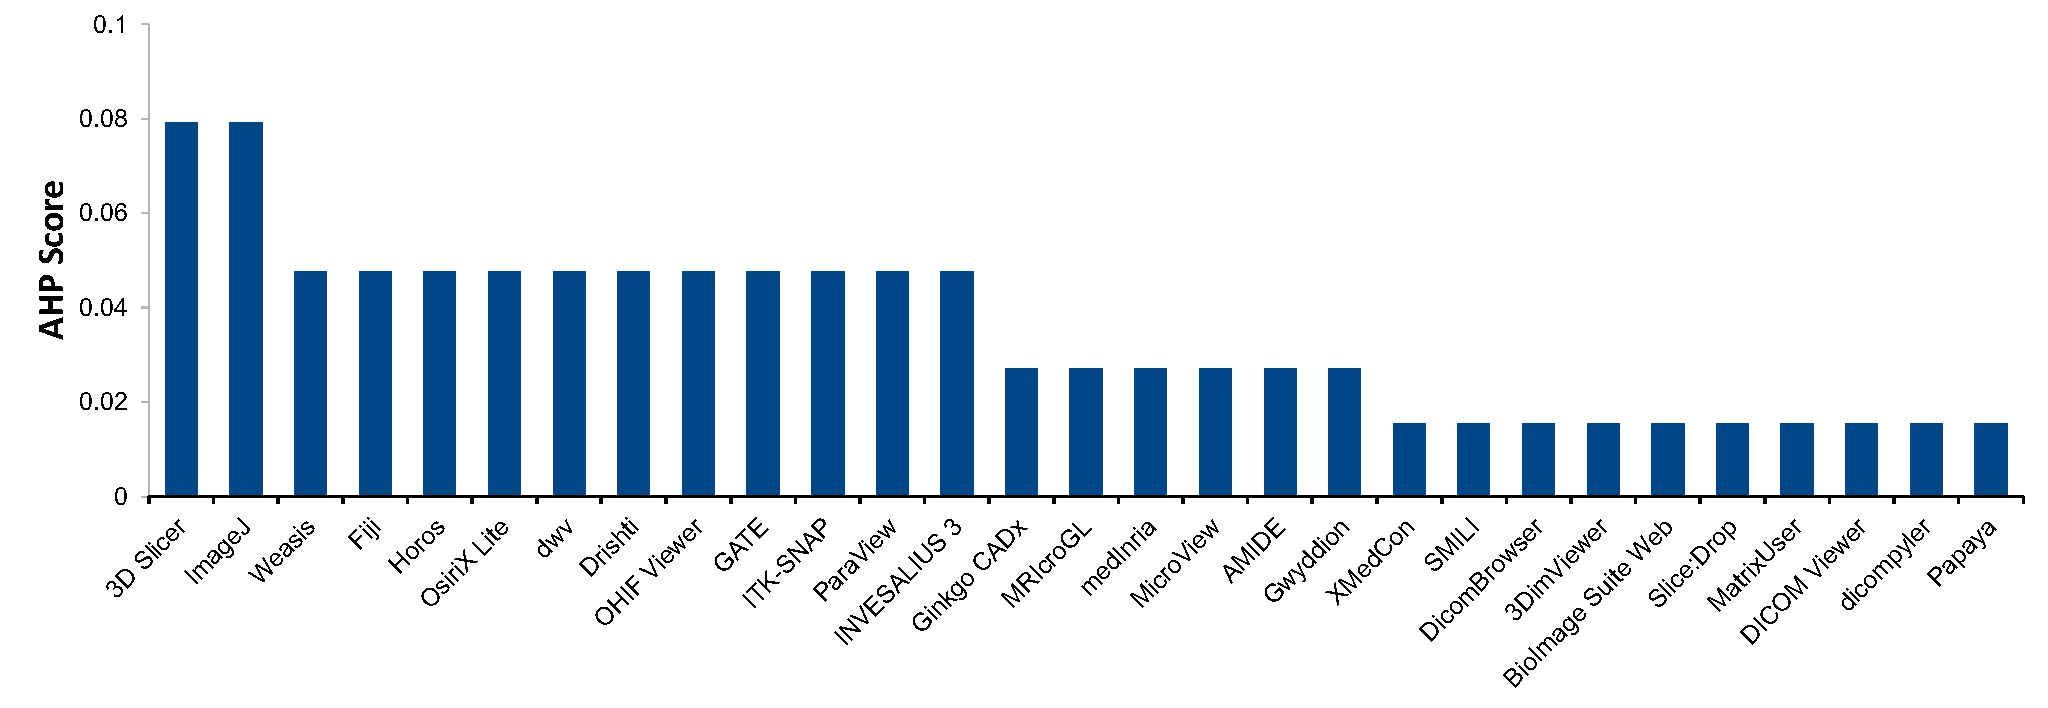
\includegraphics[scale=0.38]{understandability_scores.pdf}
\caption{AHP surface understandability scores}
\label{fg_surface_understandability_scores}
\end{figure}

\subsection{Visibility/Transparency} \label{sec_result_visibility_transparency}

Figure~\ref{fg_visibility_transparency_scores} shows the AHP scores for
visibility/transparency. Generally speaking, the teams that actively documented
their development process and plans scored higher.
Table~\ref{tab_Visibility/Transparency_docs} shows the projects that had
documents for the development process, project status, development environment,
and release notes.

\begin{figure}[ht]
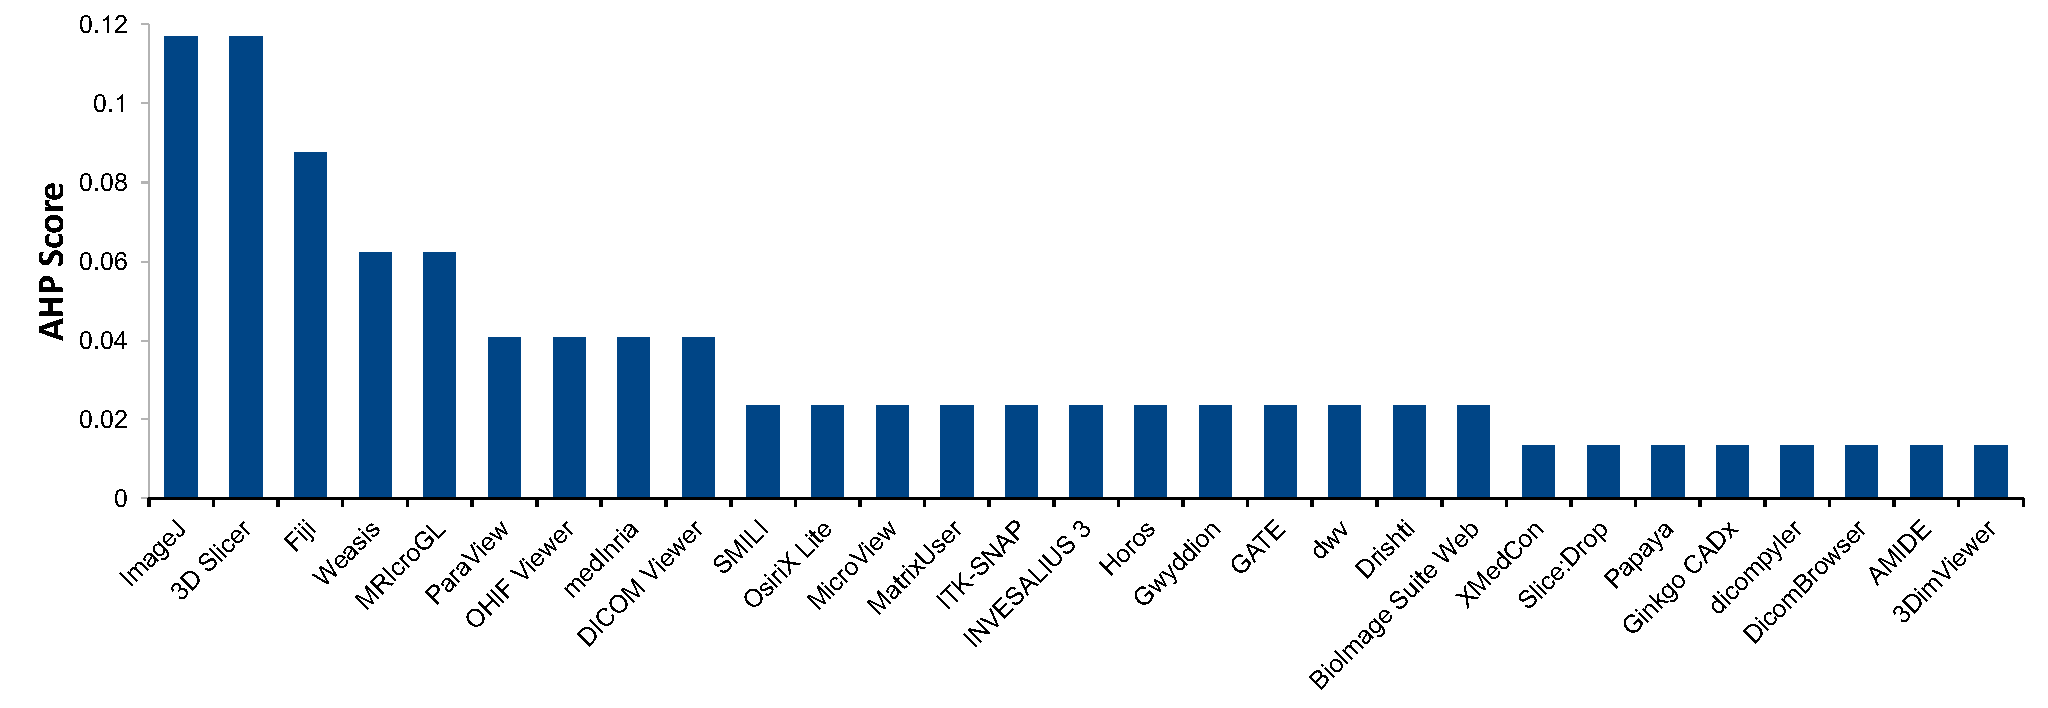
\includegraphics[scale=0.38]{visibility_transparency_scores.pdf}
\caption{AHP visibility/transparency scores}
\label{fg_visibility_transparency_scores}
\end{figure}

\begin{table}[!ht]
\centering
\begin{tabular}{lllll}
\toprule
Software & Dev.\ Process & Proj.\ Status & Dev.\ Env. & Rls.\ Notes \\ 
\midrule
3D Slicer & \checkmark & \checkmark & \checkmark & \checkmark \\
ImageJ & \checkmark & \checkmark & \checkmark & \checkmark \\
Fiji & \checkmark & \checkmark & \checkmark &  \\
MRIcroGL &  &  &  & \checkmark \\
Weasis &  &  & \checkmark & \checkmark \\
ParaView &  & \checkmark &  &  \\
OHIF Viewer &  &  & \checkmark & \checkmark \\
DICOM Viewer &  &  & \checkmark & \checkmark \\
medInria &  &  & \checkmark & \checkmark \\
SMILI &  &  &  & \checkmark \\
Drishti &  &  &  & \checkmark \\
INVESALIUS 3 &  &  &  & \checkmark \\
OsiriX Lite &  &  &  & \checkmark \\
GATE &  &  &  & \checkmark \\
MicroView &  &  &  & \checkmark \\
MatrixUser &  &  &  & \checkmark \\
BioImage Suite Web &  &  & \checkmark &  \\
ITK-SNAP &  &  &  & \checkmark \\
Horos &  &  &  & \checkmark \\
dwv &  &  &  & \checkmark \\
Gwyddion &  &  &  & \checkmark \\ 
\bottomrule
\end{tabular}
\caption{Software with visibility/transparency related documents (listed in
descending order of visibility/transparency score)}
\label{tab_Visibility/Transparency_docs}
\end{table}

\subsection{Overall Scores} \label{Sec_OverallQ}

In the absence of
a specific real world context, we assumed all nine qualities are equally
important. Figure~\ref{fg_overall_scores} shows the overall scores in descending
order.

\begin{figure}[!ht]
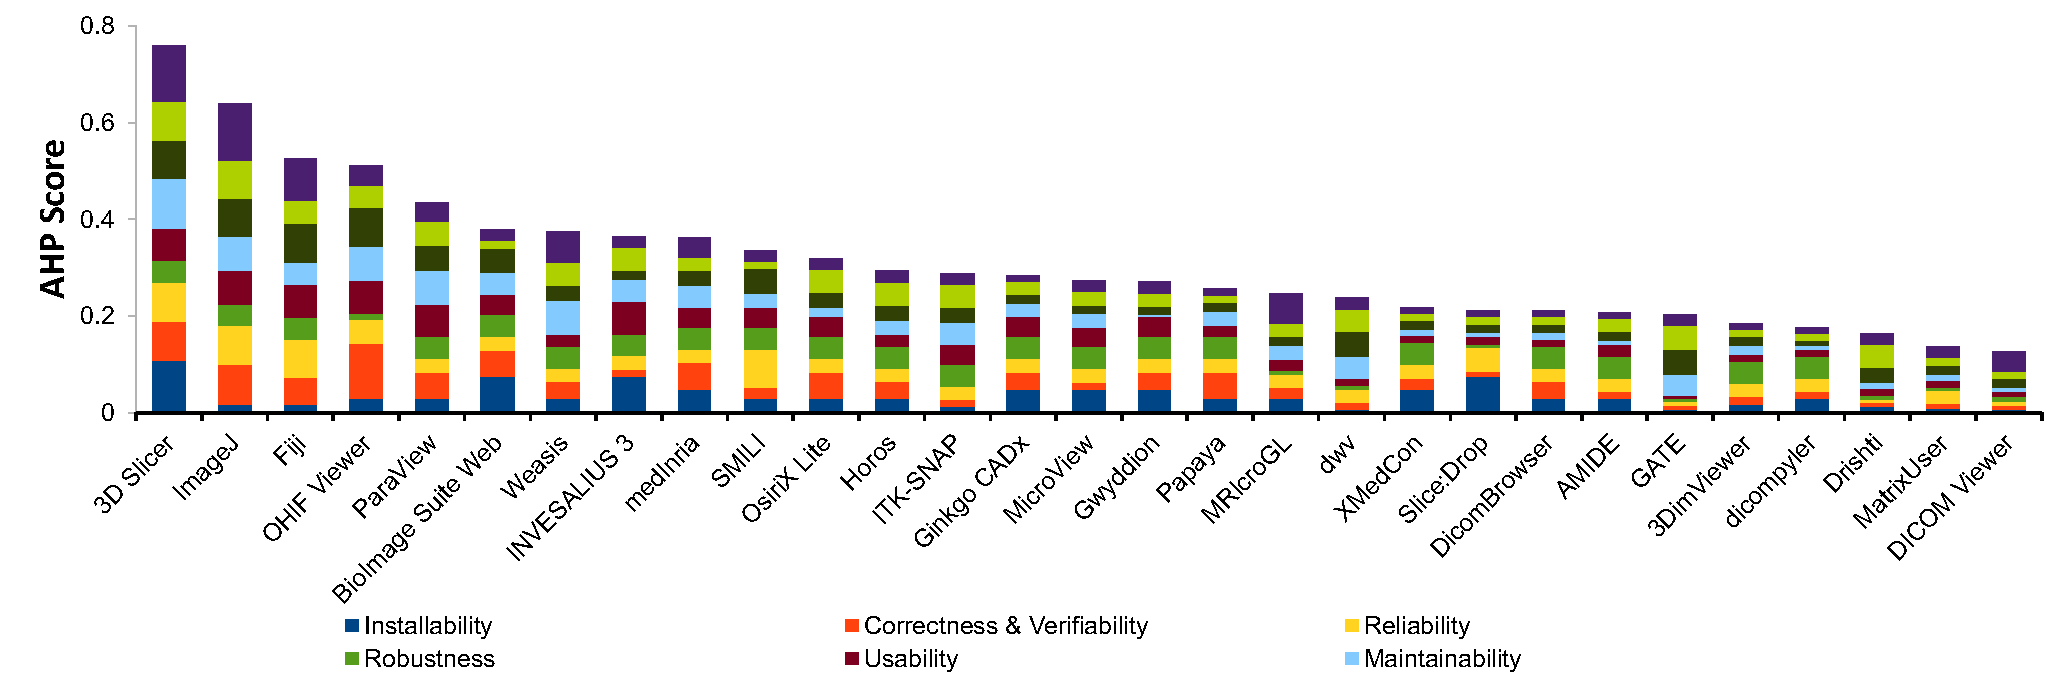
\includegraphics[scale=0.38]{overall_scores.pdf}
\caption{Overall AHP scores with an equal weighting for all 9 software qualities}

\label{fg_overall_scores}
\end{figure}

The top four software products \textit{3D Slicer}, \textit{ImageJ},
\textit{Fiji}, and \textit{OHIF Viewer} have higher scores in most criteria.
\textit{3D Slicer} has a score in the top two for all qualities; \textit{ImageJ}
ranks near the top for all qualities, except for correctness \& verifiability.
\textit{OHIF Viewer} and \textit{Fiji} have similar overall scores, with
\textit{Fiji} doing better in installability and \textit{OHIF Viewer} doing
better in correctness \& verifiability.  Given the installation problems, we may
have underestimated the scores on reliability and robustness for \textit{DICOM
Viewer}, but we compared it equally for the other seven qualities.

\section{Discussion}

We first compare our ranking to a (proxy for) the community's ranking. We then
compare the state of the practice for MI with that of other research software.
In particular we provide details on recommended artifacts that are rarely observed
for MI software. Section~\ref{sec_threats_to_validity} presents threats to the
validity of our data and conclusions.

\subsection{Comparison to Community Ranking} \label{Sec_VsCommunityRanking}

We use GitHub stars, number of forks and number of people watching the projects
are proxies for community ranking -- see Table~\ref{tab_ranking_vs_GitHub}
for statistics collected in July 2021.  Recall that 24 projects use GitHub.
Our ranking and GitHub popularity, at least for the top five projects,
seems to line up fairly well.

We ranked some popular packages fairly low, such as \textit{dwv}. This is
because we were unable to build it locally, even though we followed its
installation instructions. However, we were able to use its web
version for the rest of the measurements. Additionally, this version 
did not detect a broken DICOM file and instead displayed a blank image
(Section~\ref{sec_result_robustness}).
\textit{DICOM Viewer} ranked low as we were unable to install the
NextCloud platform.

Another likely reason for discrepancies is that we weighted all qualities
equally. This is not likely how users implicitly rank the different qualities.
This would require a broader user study to properly assess. Furthermore our
measures of popularity are only \emph{proxies} which are biased towards
past rather than current preferences~\cite{Szulik2017}, as these are
monotonically increasing quantities. Finally there are often more factors than
just quality that influence the popularity of ``consumer'' products.

\begingroup
\renewcommand{\arraystretch}{0.85}
\begin{table}[!ht]
\centering
\begin{tabular}{llllll}
\toprule
Software & Comm.\ Rank & Our Rank & Stars/yr & Watches/yr & Forks/yr \\ 
\midrule
3D Slicer & 1 & 1 & 284 & 19 & 128 \\
OHIF Viewer & 2 & 4 & 277 & 19 & 224 \\
dwv & 3 & 19 & 124 & 12 & 51 \\
ImageJ & 4 & 2 & 84 & 9 & 30 \\
ParaView & 5 & 5 & 67 & 7 & 28 \\
Horos & 6 & 12 & 49 & 9 & 18 \\
Papaya & 7 & 17 & 45 & 5 & 20 \\
Fiji & 8 & 3 & 44 & 5 & 21 \\
DICOM Viewer & 9 & 29 & 43 & 6 & 9 \\
INVESALIUS 3 & 10 & 8 & 40 & 4 & 17 \\
Weasis & 11 & 7 & 36 & 5 & 19 \\
dicompyler & 12 & 26 & 35 & 5 & 14 \\
OsiriX Lite & 13 & 11 & 34 & 9 & 24 \\
MRIcroGL & 14 & 18 & 24 & 3 & 3 \\
GATE & 15 & 24 & 19 & 6 & 26 \\
Ginkgo CADx & 16 & 14 & 19 & 4 & 6 \\
BioImage Suite Web & 17 & 6 & 18 & 5 & 7 \\
Drishti & 18 & 27 & 16 & 4 & 4 \\
Slice:Drop & 19 & 21 & 10 & 2 & 5 \\
ITK-SNAP & 20 & 13 & 9 & 1 & 4 \\
medInria & 21 & 9 & 7 & 3 & 6 \\
SMILI & 22 & 10 & 3 & 1 & 2 \\
MatrixUser & 23 & 28 & 2 & 0 & 0 \\
MicroView & 24 & 15 & 1 & 1 & 1 \\
Gwyddion & 25 & 16 & n/a & n/a & n/a \\
XMedCon & 26 & 20 & n/a & n/a & n/a \\
DicomBrowser & 27 & 22 & n/a & n/a & n/a \\
AMIDE & 28 & 23 & n/a & n/a & n/a \\
3DimViewer & 29 & 25 & n/a & n/a & n/a \\ 
\bottomrule
\end{tabular}
\caption{Software ranking by our methodology versus the community (Comm.)\
ranking using GitHub metrics (Sorted in descending order of community
popularity, as estimated by the number of new stars per year)}
\label{tab_ranking_vs_GitHub}
\end{table}
\endgroup

Although both rankings are imperfect measures, they nevertheless suggest a
correlation between best practices and popularity. We don't know if this is
causal, in either direction (i.e. if best practices enable popularity or if
popularity increases the need for using more software development best
practices).

\subsection{Software Artifacts}
\label{Sec_CompareArtifacts}

We use nine research software development guidelines to compare recommended 
software artifacts versus those present in MI software.
These guidelines are:
\begin{itemize}
\item United States Geological Survey Software Planning Checklist
\cite{USGS2019},
\item DLR (German Aerospace Centre) Software Engineering Guidelines
\cite{TobiasEtAl2018}, 
\item Scottish Covid-19 Response Consortium Software Checklist
\cite{BrettEtAl2021},
\item Good Enough Practices in Scientific Computing \cite{WilsonEtAl2016},
\item xSDK (Extreme-scale Scientific Software Development Kit) Community Package
Policies \cite{SmithAndRoscoe2018},
\item Trilinos Developers Guide \cite{HerouxEtAl2008},
\item EURISE (European Research Infrastructure Software Engineers') Network
Technical Reference \cite{ThielEtAl2020},
\item CLARIAH (Common Lab Research Infrastructure for the Arts and Humanities)
Guidelines for Software Quality \cite{vanGompelEtAl2016}, and
\item A Set of Common Software Quality Assurance Baseline Criteria for Research
Projects \cite{OrvizEtAl2017}.
\end{itemize}

\begin{table}[ht]
%\begin{center}
\begin{tabular}{ p{2.5cm}p{0.5cm}p{0.5cm}p{0.5cm}p{0.5cm}p{0.5cm}p{0.5cm}p{0.5cm}p{0.5cm}p{0.5cm}p{0.5cm} }
\toprule
~ \ & \cite{USGS2019} & \cite{TobiasEtAl2018} & \cite{BrettEtAl2021} &
\cite{WilsonEtAl2016} & \cite{SmithAndRoscoe2018} & \cite{HerouxEtAl2008} &
\cite{ThielEtAl2020} & \cite{vanGompelEtAl2016} & \cite{OrvizEtAl2017} & MI\\
\midrule
LICENSE & \checkmark & \checkmark & \checkmark & \checkmark & \checkmark & &
\checkmark & \checkmark & \checkmark & C\\
README &  & \checkmark & \checkmark & \checkmark & \checkmark & & \checkmark &
\checkmark & \checkmark & C\\
CONTRIBUTING &  & \checkmark & \checkmark & \checkmark & \checkmark & &
\checkmark & \checkmark & \checkmark & R\\
CITATION &  &  &  & \checkmark & & & & \checkmark & \checkmark & U\\
CHANGELOG &  & \checkmark &  & \checkmark & \checkmark & & \checkmark &  &  & U\\
INSTALL &  &  &  &  & \checkmark & & \checkmark & \checkmark & \checkmark & U\\
\midrule
Uninstall &  &  &  &  & & & & \checkmark & &  \\
Dependency List &  &  & \checkmark & & \checkmark & & & \checkmark &  & R\\
Authors &  &  &  &  &  &  & \checkmark & \checkmark & \checkmark & U\\
Code of Conduct &  &  &  &  & & & \checkmark & & & R\\
Acknowledgements &  &  &  &  &  &  & \checkmark & \checkmark & \checkmark & U\\
Code Style Guide &  & \checkmark &  &  & & & \checkmark & \checkmark & \checkmark & R\\
Release Info. &  & \checkmark &  &  & & \checkmark & \checkmark & & & C\\
Prod.\ Roadmap &  &  &  &  & & \checkmark & \checkmark & \checkmark & & R\\
\midrule
Getting started &  &  &  &  & \checkmark & & \checkmark & \checkmark & \checkmark & R\\
User manual &  &  & \checkmark &  & & & \checkmark & & & C\\
Tutorials &  &  &  &  & & & \checkmark & & & U\\
FAQ &  &  &  &  & & & \checkmark & \checkmark & \checkmark & U\\
\midrule
Issue Track &  & \checkmark & \checkmark & & \checkmark & \checkmark &
\checkmark & & \checkmark & C\\
Version Control &  & \checkmark & \checkmark & \checkmark & \checkmark &
\checkmark & \checkmark & \checkmark & \checkmark & C\\ 
Build Scripts &  & \checkmark &  & \checkmark & \checkmark & \checkmark &
\checkmark & & \checkmark & U\\
\midrule
Requirements &  & \checkmark &  &  & & \checkmark &  &  & \checkmark & R\\
Design Doc.\ &  & \checkmark  & \checkmark &  & \checkmark & & \checkmark &
\checkmark& \checkmark & R\\
API Doc. &  &  &  &  & \checkmark & & \checkmark & \checkmark & \checkmark & R\\
Test Plan &  & \checkmark &  &  & & \checkmark & & & &  \\
Test Cases & \checkmark & \checkmark & \checkmark &  & \checkmark & \checkmark &
\checkmark & \checkmark & \checkmark & U\\
\bottomrule
\end{tabular}
\caption{Comparison of Recommended Artifacts in Software Development Guidelines
to Artifacts in MI Projects (C for Common, U for Uncommon and R for Rare)}
\label{Tbl_Guidelines}
%\end{center}
\end{table}

In Table~\ref{Tbl_Guidelines} each row corresponds to an artifact.  For a given
row, a checkmark in one of the columns means that the corresponding guideline
recommends this artifact.  The last column shows whether the artifact appears in
the measured set of MI software, either not at all (blank), commonly (C),
uncommonly (U) or rarely (R).  We did our best to interpret the meaning of each
artifact consistently between guidelines and specific MI software, but the
terminology and the contents of artifacts are not standardized.  The challenge
even exists for the ubiquitous README file.  The content of README files shows
significant variation between projects \cite{PranaEtAl2018}.  Although some
content is reasonably consistent, with 97\% of README files contain at least one
section describing the `What' of the repository and 89\% offering some `How'
content, other categories are more variable.  For instance, information on
`Contribution', `Why', and `Who', appear in 28\%, 26\% and 53\% of the analyzed
files, respectively \cite{PranaEtAl2018}.  

\begin{table}[ht!]
    %\begin{center}
    \begin{tabular}{ p{3.1 cm} p{5.4 cm} p{3.5 cm}}
    \toprule
    Common & Uncommon & Rare \\
    \midrule
    README (29) & Build scripts (18) & Getting Started (9)\\
    Version control (29) & Tutorials (18) & Developer's manual (8)\\
    License (28) & Installation guide (16) & Contributing (8)\\
    Issue tracker (28) & Test cases (15) & API documentation (7)\\
    User manual (22) & Authors (14) & Dependency list (7)\\
    Release info. (22) & Frequently Asked Questions (FAQ) (14) & Troubleshooting guide (6)\\
     & Acknowledgements (12) & Product roadmap (5)\\
     & Changelog (12) & Design documentation (5)\\
     & Citation (11) & Code style guide (3)\\
     & & Code of conduct (1)\\
     & & Requirements (1)\\
    \bottomrule
    \end{tabular}
    \caption{Artifacts Present in MI Packages, Classified by Frequency (The number 
    in brackets is the number of occurrences)}
    \label{artifactspresent}
    %\end{center}
\end{table}

Table~\ref{artifactspresent} presents our measurements for MI software.
The table groups the artifacts by frequency
into categories of common (20 to 29 ($>$67\%) packages), uncommon (10 to 19
(33-67\%) packages), and rare (1 to 9 ($<$33\%) packages).
Tables~\ref{tab_maintainability_docs} and~\ref{tab_Visibility/Transparency_docs}
show the details on which projects use which types of artifacts for documents
related to maintainability and visibility, respectively.

Note that ``popularity'' in Table~\ref{Tbl_Guidelines} does no imply that these
oft recommended artifacts are the most important. Guidelines are often brief,
to encourage adoption, and thus even guidelines that mention the need for
installation instructions rarely mention uninstallation instructions.
Two items in Table~\ref{artifactspresent} do not appear in any guidelines:
\emph{Troubleshooting guide} and \emph{Developer's manual}.  However the
information within these documents overlaps with
the recommended artifacts.  Troubleshooting information often can be found in
a User Manual, while the information in a ``Developer's Manual'' is often
scattered amongst many other documents.

Three of the 26 recommended artifacts were never observed in the MI software:
i) Uninstall, ii) Test plans, and iii) Requirements. It is possible that
some of these were created but never put under version control.

Neglecting requirements documentation is unfortunately common for research
software, and MI software is no exception to this trend.  Although such
documentation is recommended by some \cite{TobiasEtAl2018, HerouxEtAl2008,
SmithAndKoothoor2016}, in practice this is rare~\cite{HeatonAndCarver2015}.
Sanders and Kelly \cite{SandersAndKelly2008} interviewed 16 scientists from 10
disciplines and found that none of the scientists created requirements
specifications, unless regulations in their field mandated such a document.
Requirements are the least commonly produced type of documentation for research
software in general \cite{Nguyen-HoanEtAl2010}. 

This is unfortunate as when scientific developers are surveyed on their pain
points, Wiese et al.~\cite{WieseEtAl2019} found that software requirements and
management is the software engineering discipline that most hurts them,
accounting for 23\% of the technical problems reported by study participants.
Further adding to the misfortune, there is a widespread perception that up-front
requirements are impossible for research software \cite{CarverEtAl2007,
SegalAndMorris2008}. Fortunately a more agile approach to requirements is
feasible~\cite{Smith2016}, and research-software specific templates
exist~\cite{SmithEtAl2007}. 

A theme emerges amongst the artifacts rarely observed in practice: they
are developer-focused (a list of library dependencies, a contributor's guide,
a developer Code of Conduct, coding style guidelines, product roadmap, design
documentation and API documentation).

Other communities use checklists to help with best practices. Examples include
checklists for merging branches~\cite{Brown2015}, for saving and sharing changes
to the project~\cite{WilsonEtAl2016}, for new and departing team
members~\cite{HerouxAndBernholdt2018}, for processes related to commits and
releases~\cite{HerouxEtAl2008} and for overall software
quality~\cite{ThielEtAl2020, SSI2022}.

MI projects fall somewhat short of recommended best practices, but are not alone
amongst research software projects. This gap has been documented
before~\cite{Storer2017,JohansonAndHasselbring2018}, and is known to cause
sustainability and reliability problems \cite{FaulkEtAl2009}, and to waste
development effort~\cite{deSouzaEtAl2019}.

\subsection{Threats to Validity} \label{sec_threats_to_validity}

We follow Ampatzoglou et al.\ \cite{AmpatzoglouEtAl2019}'s analysis of
threats to validity in software engineering secondary studies.

\subsubsection{Reliability}

A study is reliable if repeating it by another researcher, using the same
methodology, would lead to the same results~\cite{RunesonAndHost2009}.
We identify the following threats:

\begin{itemize}
\item One individual does the measures for all packages. A different
evaluator might find different results, due to differences in abilities,
experience, and biases.
\item The measurements for the full set of packages took several months (of
elapsed time).  Over this time the software repositories may have changed and
the reviewer's judgement may have drifted.
\end{itemize}

The measurement process used has previously been shown to be reasonably
reproducible.  \cite{SmithEtAl2016} reports grading five software
products by two reviewers. Their rankings were almost identical. As long as each
grader uses consistent definitions, the relative comparisons in the AHP results
will be consistent between graders.

\subsubsection{Construct Validity}

Construct validity is when the adopted metrics represent what they are intended
to measure~\cite{RunesonAndHost2009}. We have identified the following
potential issues:
\begin{itemize}
\item We make indirect measurement of software qualities since meaningful direct
measures for qualities like maintainability, reusability and verifiability, are
unavailable.  We follow the usual assumption that developers achieve higher
quality by following procedures and adhering to standards \cite[p.\
112]{VanVliet2000}.
\item We could not install or build \textit{dwv}, \textit{GATE}, and
\textit{DICOM Viewer}. We used a deployed on-line version for \textit{dwv}, a
virtual machine version for \textit{GATE}, but no alternative for \textit{DICOM
Viewer}.
\item Robustness measurements involve only two pieces of data, leading
to limited variation in the robustness scores
(Figure~\ref{fg_robustness_scores}). Our measurement-time budget limited
what we could achieve here.
\item Our maintainability proxies (higher ratio of comments to source,
high percentage of closed issues) have not been validated.
\item While smaller modules tend to be easier to reuse, small modules are
not necessarily good modules, nor understandable modules.
\item The understandability measure relies on 10 random source code files, but
the 10 files will not necessarily be representative. 
\item Our overall AHP ranking makes the unrealistic assumption of equal
weighting.
\item We approximated popularity by stars and watches.
\item Table~\ref{Tbl_Guidelines} required judgement as
not all guidelines use the same names for artifacts that contain
essentially the same information.
\end{itemize}

\subsubsection{Internal Validity} \label{Sec_InternalValidity}

Internal validity means that discovered causal relations are trustworthy and
cannot be explained by other factors~\cite{RunesonAndHost2009}. We identify
the following:

\begin{itemize}
\item Our search (Section~\ref{ch_results}) could
have missed a relevant package.
\item Our methodology assumes that development activities
will leave a trace in the repositories, but this is not necessarily true. For
instance, we saw little evidence of requirements
(Section~\ref{Sec_CompareArtifacts}), but teams might keep this kind of
information outside their repos.
\end{itemize}

\subsubsection{External Validity}

If the results of a study can be generalized to other situations, then the
study is externally valid \cite{RunesonAndHost2009}.  In other words, we cannot
generalize our results if the development of MI software is fundamentally
different from other research software.  Although there are differences, like
the importance of data privacy for MI data, we found the approach to developing
LBM software \cite{SmithEtAl2024} and MI software to be similar.  Except for
the domain specific aspects, the trends observed in the current study are
similar to that for other research software.

\section{Conclusions} \label{ch_conclusions}

Our analysis of the state of the practice for MI domain along nine software
qualities strongly indicates that ``higher quality'' is consistent with
community ranking proxies. Although our quality measures are rather shallow, we
see this as an advantage. The shallow measures are a proxy for the importance of
\emph{first impressions} for software adoption.

\begin{table}[ht!]
	%\begin{center}
	\renewcommand{\arraystretch}{1.8}
	\begin{tabular}{ p{2.3cm}p{9.9cm} }
		\toprule

		Quality & Ranked 1st or 2nd\\

		\midrule

		Installability & 3D Slicer, BioImage Suite Web, Slice:Drop, INVESALIUS\\

		\pbox{3.0cm}{Correctness \\ and Verifiability} & OHIF Viewer, 3D
		Slicer, ImageJ\\

		Reliability & SMILI, ImageJ, Fiji, 3D Slicer, Slice:Drop, OHIF
		Viewer\\

		Robustness & XMedCon, Weasis, SMILI, ParaView, OsiriX Lite,
		MicroView, medInria, ITK-SNAP, INVESALIUS, ImageJ, Horos, Gwyddion,
		Fiji, dicompyler, DicomBrowser, BioImage Suite Web, AMIDE, 3DimViewer,
		3D Slicer, OHIF Viewer, DICOM Viewer\\

		Usability & 3D Slicer, ImageJ, Fiji, OHIF Viewer, ParaView,
		INVESALIUS, Ginkgo CADx, SMILI, OsiriX Lite, BioImage Suite Web,
		ITK-SNAP, medInria, MicroView, Gwyddion\\

		Maintainability & 3D Slicer, Weasis, ImageJ, OHIF Viewer, ParaView\\

		Reusability & 3D Slicer, ImageJ, Fiji, OHIF Viewer, SMILI, dwv, BioImage
		Suite Web, GATE, ParaView\\

		\pbox{3.0cm}{Understandability} & 3D Slicer, ImageJ, Weasis,
		Fiji, Horos, OsiriX Lite, dwv, Drishti, OHIF Viewer, GATE, ITK-SNAP,
		ParaView, INVESALIUS\\

		\pbox{3.0cm}{Visibility and \\Transparency} & ImageJ, 3D Slicer, Fiji\\

		Overall Quality & 3D Slicer, ImageJ\\

		\bottomrule		
	\end{tabular}
	\caption{Top performers for each quality (sorted by order of quality
	measurement)} \label{topperformerstable}
	%\end{center}
\end{table} 

Our grading scores indicate that
\textit{3D Slicer}, \textit{ImageJ}, \textit{Fiji}
and \textit{OHIF Viewer} are the overall top four.  However, the
separation between the top performers and the others is not extreme.  Almost
all packages do well on at least a few qualities, as shown in
Table~\ref{topperformerstable}, which summarizes the packages ranked first and
second for each quality. Almost 70\% (20 of 29) of the software packages appear
in the top two for at least two qualities.  The only packages that do not appear
in Table~\ref{topperformerstable}, or only appear once, are \textit{Papaya},
\textit{MatrixUser}, \textit{MRIcroGL}, \textit{XMedCon}, \textit{dicompyler},
\textit{DicomBrowser}, \textit{AMIDE}, \textit{3DimViewer}, and
\textit{Drishti}.

While we did find a reasonable amount of documentation, especially when
consider all MI projects, there were definitely some holes. Some important
documentation (test plans and requirements documentation) was missing,
and other (contributors' guide, code of conduct, code style guidelines, product
roadmap, design documentation, and API documentation)
(Section~\ref{Sec_CompareArtifacts}) were rare.

A deeper understanding of the needs of
the MI community will require data beyond what is available in
repositories.  Future work should involve interviewing MI developers to
better understand their ``pain points''.

\section*{Acknowledgements}

We would like to thank Peter Michalski and Oluwaseun Owojaiye for fruitful
discussions on topics relevant to this paper.

\section*{Conflict of Interest}

On behalf of all authors, the corresponding author states that there is no
conflict of interest.

\bibliography{SOP_MI_OSR}

\end{document}
